\documentclass[t,usenames,dvipsnames]{beamer}
\usetheme{Copenhagen}
\setbeamertemplate{headline}{} % remove toc from headers
\beamertemplatenavigationsymbolsempty

\usepackage{amsmath, sfmath, tikz, xcolor, pgfplots, array}
\pgfplotsset{compat = 1.16}
\usetikzlibrary{arrows.meta, calc, decorations.pathreplacing}

\title{Parabolas}
\author{}
\date{}

\AtBeginSection[]
{
  \begin{frame}
    \frametitle{Table of Contents}
    \tableofcontents[currentsection]
  \end{frame}
}

\begin{document}

\begin{frame}
    \maketitle
\end{frame}

\section{Find the vertex, focus, and directrix for a parabola in standard form.}

\begin{frame}{Intro}
If we look at the graph of the quadratic function $f(x) = ax^2 + bx + c$, we obtain what is known as a \emph{parabola}.    \newline\\    \pause

A \alert{parabola} is the set of all points in the plane that are the same distance from the focus and the directrix line.
\end{frame}

\begin{frame}{}
\begin{center}
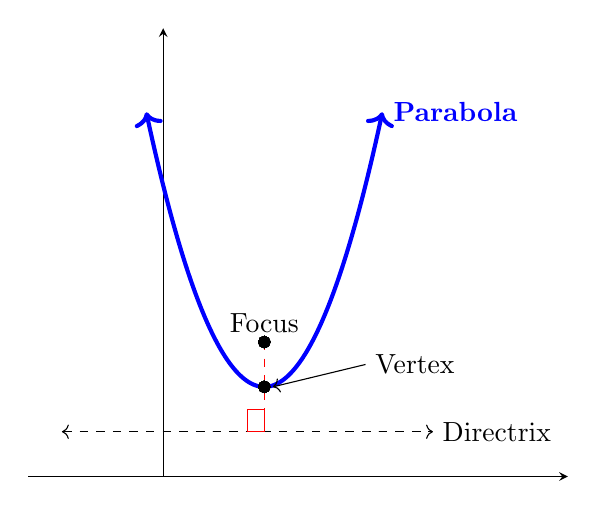
\begin{tikzpicture}
    \begin{axis}[
    axis lines = middle,
    xmin = -4,
    xmax = 12,
    ymin = 0,
    ymax = 10,
    xtick = \empty,
    ytick = \empty]
    \addplot [color=blue, <->, samples=200, domain=-0.5:6.5, line width = 1.5] {2 + 0.5*(x-3)^2} node[right]{\color{blue}{\textbf{Parabola}}};
    \addplot [mark = *] (3, 3) node[above]{Focus};
    \addplot [dashed, <->, samples=200, domain = -3:8] {1} node[right]{Directrix};
    \addplot [mark = *] (3, 2);
    \draw [<-] (3.25,2) -- (6,2.5) node[right]{Vertex};
    \draw [color=red] (3,1) rectangle (2.5,1.5);
    \draw [color=red, dashed] (3,3) -- (3,2) -- (3,1);
    \end{axis}
\end{tikzpicture}
\end{center}
\pause

The \alert{focal length} is the distance between the focus and vertex (or directrix and vertex) and is $|p|$.
\end{frame}

\begin{frame}{Equations}
    \begin{center}
    \setlength{\extrarowheight}{5pt}
    \begin{tabular}{c|c|c}
    &   \textbf{Opens Up or Down}   &   \onslide<2->{\textbf{Opens Left or Right}}    \\  \hline
    &   $(x-h)^2 = 4p(y-k)$  &   \onslide<2->{$(y-k)^2 = 4p(x-h)$}  \\[5pt]  \hline
    Vertex  &   $(h,k)$ &   \onslide<2->{$(h,k)$} \\[5pt]  \hline
    Focus Point   &   $(h, k+p)$    &   \onslide<2->{$(h+p, k)$}  \\[5pt] \hline
    Directrix   &   $y = k-p$   &   \onslide<2->{$x = h-p$}   \\
    \end{tabular}
\end{center}
\vspace{11pt}
\onslide<3->{
\emph{Note}: Sometimes the equations are written as 
\[y = \frac{1}{4p}(x-h)^2 + k \text{ and } x = \frac{1}{4p}(y-k)^2 + h\].}
\end{frame}

\begin{frame}{Finding Vertex Without Technology}
    For $y = ax^2 + bx + c$  \\[8pt] \pause
    \begin{enumerate}
        \item $x$-coordinate: $-\frac{b}{2a}$   \\[8pt]   \pause
        \item $y$-coordinate: Evaluate at $x$-coordinate \\[18pt] \pause
    \end{enumerate}
    
    For $x = ay^2 + by + c$ \\[8pt] \pause
    \begin{enumerate}
        \item $y$-coordinate: $-\frac{b}{2a}$   \\[8pt] \pause
        \item $x$-coordinate: Evaluate at $y$-coordinate
    \end{enumerate}
\end{frame}

\begin{frame}{Example 1}
Find the vertex, focus, and directrix line for $(x+1)^2 = -8(y-3)$. \pause
Graph the parabola: \newline\\
\begin{minipage}{0.5\textwidth}
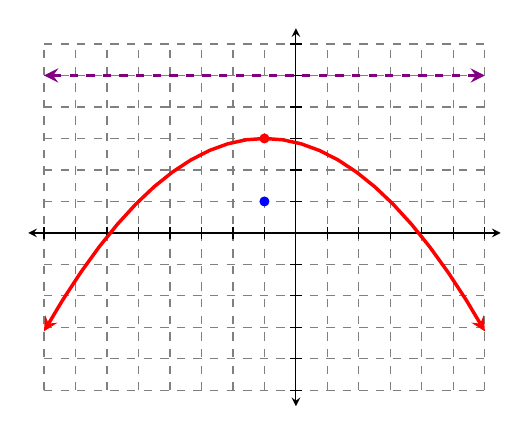
\begin{tikzpicture}[scale=0.4]
    \draw [color=gray, dashed] (-8,-5) grid (6,6);
    \draw [<->, >=stealth] (-8.5,0) -- (6.5,0);
    \draw [<->, >=stealth] (0,-5.5) -- (0,6.5);
    \foreach \x in {-8,-7,...,6}
    \draw (\x, 0.2) -- (\x,-0.2);
    \foreach \y in {-5,-4,...,6}
    \draw (0.2,\y) -- (-0.2,\y);
    \draw [<->, >=stealth, domain=-8:6, color=red, line width = 1.25] plot (\x, {-0.125*(\x+1)*(\x+1)+3});
    \onslide<3->{\draw[color=red, fill=red] (-1,3) circle (4pt);}
    \onslide<8->{\draw[color=blue, fill=blue] (-1,1) circle (4pt);}
    \onslide<10->{\draw[color=violet, <->, >=stealth, line width=1.25, dashed] (-8,5) -- (6,5);}
\end{tikzpicture}
\end{minipage}
\hspace{0.5cm}
\begin{minipage}{0.4\textwidth}
\onslide<4->{Vertex: $(-1,3)$} \\[8pt]
\onslide<5->{$4p = |-8|$} \\[8pt]
\onslide<6->{$p = 2$} \\[8pt]
\onslide<7->{Focus: $(-1, 3-2)$} \\[8pt]
\onslide<8->{Focus: $(-1,1)$} \\[8pt]
\onslide<9->{Directrix: $y = 3 + 2$} \\[8pt]
\onslide<10->{Directrix: $y = 5$} 
\end{minipage}
\end{frame}


\begin{frame}{Example 2}
Find the vertex, focus, and directrix for $(y-2)^2 = 12(x+1)$.  \newline\\
\pause
\begin{minipage}{0.4\textwidth}
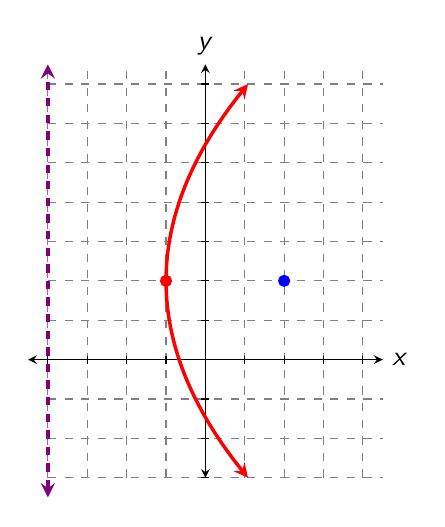
\begin{tikzpicture}[scale=0.5]
    \draw [dashed, gray] (-4,-3) grid (4.5,7.5);
      \draw[<->, >=stealth] (-4.5,0) -- (4.5,0) node[right] {$x$};
      \draw[<->, >=stealth] (0,-3) -- (0,7.5) node[above] {$y$};
      \foreach \x in {-4,-3,-2,...,4}
      \draw (\x, 0.1) -- (\x, -0.1);
      \foreach \y in {-3,-2,...,7}
      \draw (0.1,\y) -- (-0.1,\y);
      \draw[<->, >=stealth, line width = 1.25, domain=-3:7,smooth,variable=\y,red]  plot ({0.0833*\y*\y - 0.333*\y - 0.667},\y);
      \draw [color=red, fill=red] (-1,2) circle (4pt);
      \onslide<6->{\draw[color=blue, fill=blue] (2,2) circle (4pt);}
      \onslide<7->{\draw[<->,>=stealth, line width = 1.25, dashed, color=violet] (-4,-3.5) -- (-4,7.5);}
    \end{tikzpicture}
\end{minipage}
\hspace{0.6cm}
\begin{minipage}{0.48\textwidth}
\onslide<3->{Vertex: $(-2,1)$} \\[10pt]
\onslide<4->{$4p = 12$} \\[10pt]
\onslide<5->{$p = 3$} \\[10pt]
\onslide<6->{Focus: $(-1+3, 2) \rightarrow (2,2)$} \\[10pt]
\onslide<7->{Directrix: $x = -1-3$} \\[10pt]
\onslide<8->{$x = -4$} \\
\end{minipage}
\end{frame}

\section{Find the equation of the standard form of a parabola.}

\begin{frame}{Latus Rectum and Focal Diameter}
The \alert{latus rectum} of a parabola is a line segment through the focus point that is parallel to the directrix line.   \newline\\
\pause
The \alert{focal diameter} is the length of the latus rectum, and is $\mid 4p \mid$.  \newline\\
\pause
\begin{center}
    \begin{tikzpicture}[scale=0.8]
    \begin{axis}[
    axis lines = middle,
    xmin = -4,
    xmax = 12,
    ymin = 0,
    ymax = 10,
    xtick = \empty,
    ytick = \empty]
    \addplot [color=blue, <->, samples=200, domain=-0.5:6.5, line width = 1.5] {1 + 0.5*(x-3)^2};
    \addplot [mark = *] (3, 3);
    \addplot [dashed, domain=1:5, line width = 1.25] {3} node [midway, above, yshift=0.2cm] {L.R.};
    \draw [decoration = {brace}, decorate] (1,3.2) -- (5,3.2);
    \end{axis}
    \end{tikzpicture}
\end{center}
\end{frame}

\begin{frame}{Example 3}
Find the standard form of the parabola with focus $(2, 1)$ and directrix $y = -4$.   \newline\\
\begin{minipage}{0.6\textwidth}
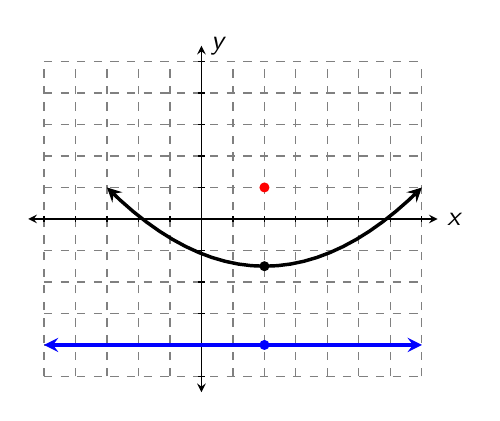
\begin{tikzpicture}[scale=0.4]
\draw [gray, dashed] (-5,-5) grid (7,5);
\draw [<->, >=stealth] (-5.5,0) -- (7.5,0) node [right] {$x$};
\draw [<->, >=stealth] (0,-5.5) -- (0,5.5) node [right] {$y$};
\foreach \x in {-5,-4,...,7}
\draw (\x, 0.1) -- (\x, -0.1);
\foreach \y in {-5,-4,...,5}
\draw (0.1,\y) -- (-0.1,\y);
\draw [<->, >=stealth, color=blue, line width = 1.25] (-5,-4) -- (7,-4);
\draw [color=red, fill=red] (2,1) circle (4pt);
\onslide<2->{\draw [color=blue, fill=blue] (2,-4) circle (4pt);}
\onslide<8->{\draw [<->, >=stealth, domain = -3:7, line width = 1.25] plot (\x, {0.1*(\x-2)*(\x-2)-1.5});}
\onslide<3->{\draw [fill=black] (2,-1.5) circle (4pt);}
\end{tikzpicture}
\end{minipage}
\begin{minipage}{0.35\textwidth}
\onslide<4->{Vertex: $(2,-1.5)$}    \\[11pt]
\onslide<5->{$p = 2.5$} \\[11pt]
\onslide<6->{$4p = 10$} \\[11pt]
\onslide<7->{$(x-2)^2 = 10(y+1.5)$} \\
\end{minipage}
\end{frame}


\begin{frame}{Converting Equations}
To convert parabolas in $y = ax^2 + bx + c$ form to standard form, do the following:  \newline\\  \pause
\begin{enumerate}
    \item Find the coordinates of the vertex. This will give you $h$ and $k$.    \pause  \\[11pt]
    \item Use the relationship that $4p = \frac{1}{a}$.
\end{enumerate}    
\end{frame}

\begin{frame}{Example 4a}
Find the vertex, focus, and directrix of the following. \newline\\
(a) \quad $y^2 + 4y + 8x = 4$   \newline\\  \pause
\begin{minipage}{0.4\textwidth}
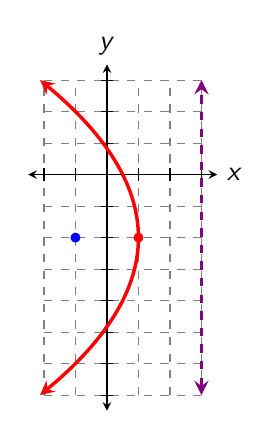
\begin{tikzpicture}[scale=0.4]
    \draw [dashed, gray] (-2,-7) grid (3,3);
      \draw[<->, >=stealth] (-2.5,0) -- (3.5,0) node[right] {$x$};
      \draw[<->, >=stealth] (0,-7.5) -- (0,3.5) node[above] {$y$};
      \foreach \x in {-2,-1,...,3}
      \draw (\x, 0.2) -- (\x, -0.2);
      \foreach \y in {-7,-6,...,3}
      \draw (0.2,\y) -- (-0.2,\y);
      \draw[<->, >=stealth, line width = 1.25, domain=-7:3,smooth,variable=\y,red]  plot ({-0.125*(\y*\y + 4*\y - 4)},\y);
      \onslide<4->{\draw[color=red,fill=red] (1,-2) circle (4pt);}
      \onslide<8->{\draw[color=blue,fill=blue] (-1,-2) circle (4pt);}
      \onslide<10->{\draw[color=violet, line width=1.25, dashed, <->, >=stealth] (3,-7) -- (3,3);}
\end{tikzpicture}
\end{minipage}
\hspace{0.25cm}
\begin{minipage}{0.4\textwidth}
\onslide<3->{Vertex: $(1,-2)$} \\[10pt]
\onslide<5->{$4p = |8|$} \\[10pt]
\onslide<6->{$p = 2$} \\[10pt]
\onslide<7->{Focus: $(1-2, -2)$} \\[10pt]
\onslide<8->{Focus: $(-1,-2)$} \\[10pt]
\onslide<9->{Directrix: $x = 1 + 2$} \\[10pt]
\onslide<10->{Directrix: $x = 3$}
\end{minipage}
\end{frame}

\begin{frame}{Example 4b}
(b) \quad $x^2 - 2x + 5y = 1$   \newline\\  \pause
\begin{minipage}{0.4\textwidth}
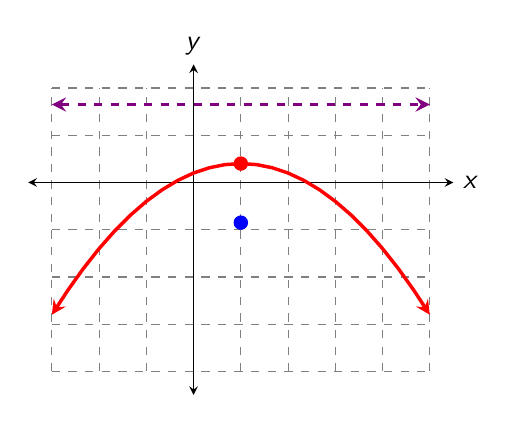
\begin{tikzpicture}[scale=0.6]
    \draw[dashed, gray] (-3,-4) grid (5,2);
    \draw[<->,>=stealth] (-3.5,0)--(5.5,0) node [right] {$x$};
    \draw[<->,>=stealth] (0,-4.5)--(0,2.5) node [above] {$y$};
    \draw[<->,>=stealth,color=red,line width=1.25,domain=-3:5] plot (\x, {-0.2*(\x-1)*(\x-1)+0.4});
    \onslide<4->{\draw[color=red,fill=red] (1,0.4) circle (4pt);}
    \onslide<8->{\draw[color=blue,fill=blue] (1,-0.85) circle (4pt);}
    \onslide<10->{\draw[color=violet,<->,>=stealth,dashed,<->,>=stealth,line width = 1.25] (-3,1.65) -- (5,1.65);}
\end{tikzpicture}
\end{minipage}
\hspace{1.5cm}
\begin{minipage}{0.4\textwidth}
\onslide<3->{Vertex: $\left(1,\frac{2}{5}\right)$} \\[8pt]
\onslide<5->{$4p = |5|$} \\[8pt]
\onslide<6->{$p = 5/4$} \\[8pt]
\onslide<7->{Focus: $\left(1, \frac{2}{5}-\frac{5}{4}\right)$} \\[8pt]
\onslide<8->{Focus: $\left(1, -\frac{17}{20}\right)$} \\[8pt]
\onslide<9->{Directrix: $y = \frac{2}{5} + \frac{5}{4}$} \\[8pt]
\onslide<10->{Directrix: $y = \frac{33}{20}$} \\
\end{minipage}
\end{frame}

\section{Applications of Parabolas}

\begin{frame}{Paraboloid}
    If we rotate a parabola around its axis of symmetry, we obtain a 3-D model of a parabola called a \alert{paraboloid}, or a \alert{paraboloid of revolution}.    \newline\\  \pause
    
    The nature of paraboloids allows signals to be sent to or from the focus in a directed manner.
\end{frame}

\begin{frame}{Example 5}
    A satellite dish is to be constructed in the shape of a paraboloid of revolution. If the receiver placed at the focus is located 2 ft above the vertex of the dish, and the dish is to be 12 feet wide, how deep will the dish be?    
\end{frame}

\begin{frame}{Example 5}
    If we place the vertex at the origin and open the graph upward, \onslide<2->{we get the equation $x^2 = 8y$}    \newline
    \begin{minipage}{0.5\textwidth}
        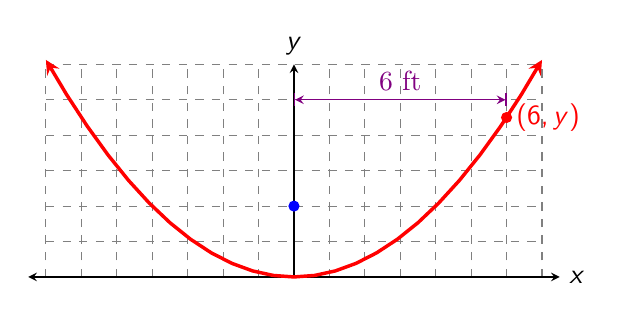
\begin{tikzpicture}[scale=0.45]
            \draw[dashed, gray] (-7,0) grid (7,6);
            \draw[<->,>=stealth] (-7.5,0) -- (7.5,0) node [right] {$x$};
            \draw[->,>=stealth] (0,0) -- (0,6) node [above] {$y$};
            \draw[<->,>=stealth,color=red,domain=-7:7,line width=1.25] plot ({\x, 0.125*\x*\x});
            \draw[color=blue,fill=blue] (0,2) circle (4pt);
            \onslide<3->{\draw[|<->|,>=stealth,color=violet] (0,5) -- (6,5) node [midway, above] {6 ft};}
            \onslide<5->{\draw[color=red,fill=red] (6,4.5) circle (4pt) node [right] {$(6,y)$};}
        \end{tikzpicture}
    \end{minipage}
    \hspace{1cm}
    \begin{minipage}{0.3\textwidth}
    \begin{align*}
        \onslide<4->{x^2 &= 8y} \\[10pt]
        \onslide<6->{6^2 &= 8y} \\[10pt]
        \onslide<7->{36 &= 8y} \\[10pt]
        \onslide<8->{y &= \frac{36}{8}} \\[10pt]
        \onslide<9->{y &= \frac{9}{2}} \\
    \end{align*}
    \end{minipage}
\end{frame}



\end{document}
